\documentclass{llncs}

\usepackage{amssymb}
\usepackage{cite}
\usepackage{times}
\usepackage{amssymb,amsmath}
\usepackage{graphicx}
\usepackage{url}

\renewcommand{\UrlFont}{\small\tt}
\renewcommand{\ttdefault}{cmtt}


\setcounter{tocdepth}{3}	
\urldef{\mailsa}\path|{v.bajpai, n.melnikov, s.anuj, j.schoenwaelder}@jacobs-university.de|
\newcommand{\keywords}[1]{\par\addvspace\baselineskip
\noindent\keywordname\enspace\ignorespaces#1}

\newenvironment{mytinylisting}
{\begin{list}{}{\setlength{\leftmargin}{1em}}\item\scriptsize\bfseries}
{\end{list}}

\newcommand{\Keywords}[1]{\par\noindent 
{\small{\em \bf{\\Keywords}\/}: #1}}

\begin{document}

\mainmatter  % start of an individual contribution

\title{Flow-based Identification of Failures\\
  Caused by IPv6 Transition Mechanisms}

\author{Vaibhav Bajpai, Nikolay Melnikov, Anuj Sehgal and J\"urgen Sch\"onw\"alder}
\institute{Computer Science, Jacobs University Bremen, Germany \\
Campus Ring 1, 28759 Bremen, Germany
\mailsa}
\titlerunning{Flow-based Identification of Failures Caused by IPv6 Transition Mechanisms}
\authorrunning{Vaibhav Bajpai, Nikolay Melnikov, Anuj Sehgal and J\"urgen Sch\"onw\"alder}
\maketitle

\begin{abstract}
The IETF has developed several solutions that promote IPv4 and IPv6 co-existence, but they need to be thoroughly tested on a large scale, before they can actually be considered as viable solutions. In the following study we present an experimental evaluation of the two popular transitioning technologies: NAT64 and Dual-Stack Lite. Our first goal is to identify how well current applications, protocols and online services interoperate with these technologies and to detect their potential failures. Our second goal is to use a stream-oriented flow query language NFQL, to formulate queries that can find those failures by scanning through traces of NetFlow records. We identified several applications that fail under NAT64, and we analyze how to detect these failures in an automated fashion.

\Keywords{IPv6, Transition, NAT64, Dual-Stack Lite, NetFlow}
\end{abstract}

\section{Motivation}
\label{sec:introduction}

The IETF began work on IPv6 in the mid 1990s realizing that it would not take long for the IPv4 address space to run out, given the pace of Internet adoption and growth. By the mid 1990s IPv6 was defined, but it did little to displace IPv4 as the de facto standard. This has been due to the lack of any economic advantage for the network providers to deploy IPv6 and a lack of IPv6-only killer applications that can aggressively push the need for end users to look for any service benefit to make the switch. Studies show that IPv6 (as of February 2012) accounts for less than 1\% of the global Internet traffic and only about 0.5\% of the top 1 million websites are reachable over IPv6 \cite{ipv6monitor}. 

Today, the issue of depleting IPv4 addresses has become more imminent and undeniable. APNIC announced that it had reached the final stage of IPv4 exhaustion in the Asia Pacific region with the release of all IPv4 addresses in its available pool \cite{APNIC}. This occurred only few months after IANA allocated the last blocks of IPv4 addresses to the Internet Registries exhausting its pool of unallocated IPv4 addresses \cite{iana}. Despite the foresight on the rapid decline, IPv6 is still in the very early stages of deployment. Very few network operators, even those with aggressive deployment plans, have completed IPv6 roll outs. Most network operators have not even begun IPv6 deployment. Usually two factors are attributed to such a reluctance: the amount of currently available IPv4 content and the large number of installed applications, both at home and at enterprise networks, that do not work over IPv6, which will make the transition from IPv4 to IPv6 to take multiple years.
Therefore, the service providers and the enterprises will either need to better leverage the current pool of addresses by sharing the IPv4 addresses among many customers using wider/layered NAT deployments or employ technologies and mechanisms that allow to reach IPv4 content from IPv6-only hosts during the extended migration phase.  

The findings of this study demonstrate that many of the existing applications and protocols interoperate well with the existing transition mechanisms. These findings correspond to some of the observations made in other independent studies \cite{ARKKO, UENO, citeulike:9731000}. There are, as we found out, several applications that do not work, and these are the border-line cases that many operators and service providers are afraid of. These failures can significantly decrease users' overall experiences or satisfaction with the provided services, and this would definitely hurt the reputation of the network operator or the service provider. The goal of our study is twofold. First, we wanted to understand which applications fail under IPv6 transition mechanisms and the reasons causing these applications to fail. Second, we wanted to investigate whether it is possible to identify these failures in network flow records. If this were possible, we could create a scalable tool that can be used by network operators deploying transition technologies to detect failures customers are facing and to take appropriate actions before a customer complains about his network service. In the following, we term a sequence of flow-records that is characteristic for an application failure due to a transition technology a \emph{failure signature}. The failure signatures can be formalized by using our stream oriented flow-query language NFQL \cite{MARINOV, AIMS2010}. We assume that failure signatures are unique for each application, since each one of them performs a different sequence of network-related operations in the background. Once we understand and define what a failure signature of a certain application is, we can use that signature to automatically scan through massive amounts of flow records in order to automatically detect failures. This will allow service providers and network operators to take a proactive rather than a reactive approach to problems that users may face after deployment of transition mechanisms and this can likely mitigate some of the risks associated with the rollout of IPv6 transition technologies.

The structure of the paper is as follows. In the next section we
briefly introduce the transition technologies Dual-Stack Lite and NAT64. Section \ref{sec:netflow} gives an overview of NetFlow and our stream-oriented flow query language NFQL. Our experiments to evaluate the interoperability of different applications with DS-Lite and NAT64 are presented in Sections \ref{sec:app-ds-lite} and \ref{sec:app-nat64} respectively. In Section \ref{sec:failure-analysis}, we analyze the reasons for the failure of different applications. Related work is discussed in Section \ref{sec:related-ipv6} before we conclude in Section \ref{sec:conclusion}.

\section{Investigated IPv4-to-IPv6 Transition Technologies}
\label{sec:technology}

We concentrated our analysis on the two transition technologies DS-Lite and NAT64. Related technologies not investigated are discussed briefly in Section \ref{sec:related-ipv6}.

\subsection{Dual-Stack Lite}
\label{sec:ds-lite}
DS-Lite (Dual-Stack Lite) \cite{DSLITE} is an approach that uses IPv6-only links between the ISP (Internet Service Provider) and the customer. When a device in the customer network sends an IPv4 packet to an external destination, the IPv4 packet is encapsulated in an IPv6 packet for transport into the provider network as shown in Figure \ref{fig:MultipleDeviceDSLite}. At the CGNAT (Carrier Grade NAT), the packet is decapsulated to IPv4 and NAT44 is applied (which translates an IPv4 address to another IPv4 address) before delivering the packet to the public Internet. Using this approach, a service provider can deploy IPv6 and take advantage of its large address space while still providing IPv4 service. In particular, this technique allows a global IPv4 address to be shared among a larger set of customers. 

A DS-Lite CPE (Customer Premises Equipment) performs the IPv4-in-IPv6 encapsulation of the IPv4 packet sent by the device, setting the destination address of the IPv6 packet to the address of the DS-Lite enabled CGNAT. The CGNAT must adapt its NAT binding table to add the source address of the encapsulating IPv6 packet (the address of the customer end of the IPv6 link), the IPv4 source address and port. Such a combination makes the mapping unambiguous. As a result, when an IPv4 packet is received from outside, the IPv4 destination address and port are mapped back to the inside IPv4 destination address and port, encapsulated in IPv6 using the mapped IPv6 address as the IPv6 destination address, and then forwarded to the customer. The mapped IPv6 address not only disambiguates the customer's private address space \cite{RFC1918}, it also provides the reference for the tunnel endpoint.
\begin{figure}[t]
\centering
\includegraphics*[width=0.85\linewidth]{dslite2} 
\caption{DS-Lite: IPv4 traffic is tunneled from a customer's network   to a carried grade NAT in the provider network sharing an IPv4 address with potentially many customers}
\label{fig:MultipleDeviceDSLite}
\end{figure}
On the other hand, if a device in the customer network sends an IPv6 packet, the packet is routed normally to the IPv6 destination. In this way, this model allows use of Dual-Stacked, IPv4-only, and IPv6-only devices behind the gateway. A variation on the DS-Lite Model implements DS-Lite on an individual end system rather than on a CPE device. One critical requirement for DS-Lite is that its tunnelling function must be added to existing customers CPE either through a software upgrade or by replacing the unit.

\subsection{NAT64}
\label{sec:nat64}
An IPv4-to-IPv6 Network Address Translator (NAT64) \cite{NAT64} allows IPv6-only clients to contact IPv4 servers using unicast UDP, TCP, or ICMP. The headers of packets passing between an IPv6-only end system and an IPv4-only end system are converted from one protocol to the other using the IP/ICMP Translation Algorithm \cite{rfc6145}, allowing the end systems to communicate without knowing that the remote system is using a different IP version. A special DNS Application Level Gateway (ALG), known as DNS64 \cite{DNS64}, is used to trick IPv6 hosts into thinking that the IPv4 destination has an IPv6 address. The IPv6 host believes that it is communicating with another IPv6 system, and the IPv4 system believes that it is talking to another IPv4 system. Neither end system participates directly in the translation process. 

\begin{figure}[t]
  \centering
  \includegraphics*[width=0.85\linewidth]{nat64} 
  \caption{NAT64/DNS64: A special DNS64 server synthesizes AAAA     records out of A records and an associated NAT64 translates IPv6 packets into IPv4 packets}
  \label{fig:NAT64}
\end{figure}

The NAT64 server is the endpoint for at least one public IPv4 address and a 32-bit long IPv6 network prefix \texttt{(64:FF9B::/96)}. The IPv6 client accommodates the IPv4 address it wishes to communicate within the left-over 96-bits, and sends its packets to the resulting address. The NAT64 server then creates a NAT-mapping between the IPv6 and the IPv4 address, allowing the end-points to communicate. DNS64 describes a DNS server that, when asked for a domain's AAAA records, synthesizes them from the requested domain's A records. The first part of the synthesized IPv6 address points to an IPv6/IPv4 translator and second part embeds the IPv4 address from the A record. The translator in question is usually a NAT64 server as shown in Figure \ref{fig:NAT64}.

The most significant limitation of this architecture is that all hosts and all applications within the NAT64 domain must be converted to IPv6. Legacy IPv4 hosts or IPv4 applications running on an IPv4 host will not work in this architecture. In addition the translation only works for cases where DNS is used to find the remote host address. If IPv4 literals are used, the DNS64 server will never be involved, and hence, there is no special IPv6 address to use. DNSSEC validation will also fail since DNS64 server needs to return records not specified by the domain owner.        

\section{NetFlow and NFQL}
\label{sec:netflow}

\begin{figure}[ht!]
  \centering
  \includegraphics*[width=0.65\linewidth]{netflow-overview}	
  \caption{NetFlow: A flow exporter aggregates packets passing an observation point into flow records that are sent to a flow collector for further analysis}
  \label{fig:netflow-overview}
\end{figure}
NetFlow \cite{rfc3954} by Cisco Systems is a protocol that allows network elements to export IP flow information to designated collectors from where they can be later retrieved for further analyses. The traditional definition of a flow uses a 7-tuple key. Specifically, a flow is a unidirectional sequence of packets sharing all of the following seven values: source/destination IP addresses, source/destination ports, protocol, ingress interface, type of service field. If two IP packets differ in one of the seven fields, then they belong to different flows. In addition to the key fields, a flow contains other accounting fields which may differ slightly depending on the NetFlow version.

A high-level overview of the NetFlow protocol is shown in Figure \ref{fig:netflow-overview}. The flow exporter reads the IP packets that cross an observation point (typically a network interface of a router) to generate flow-records. The flow-records are exported based on some predefined expiration rules, such as a TCP \texttt{FIN} or \texttt{RST}, an inactivity timeout, a regular export timeout or crossing a low memory threshold. The flow-records are encapsulated in UDP datagrams and are deleted from the exporter once transmitted. On the other end, the collector on receiving these flow-records, decodes and stores them locally to be used for further processing.

The Network Flow Query Language (NFQL) \cite{jschauer:thesis:2011, AIMS2010} is a stream-based flow record query language \cite{MARINOV}. The query language allows us to describe patterns in flow-records in a declarative and orthogonal fashion, making it easy to read and flexible enough to describe complex relationships among a given set of flows. A typical query consists of several branches where each branch consists of a number of independent stages that perform a specific task.

\section{Testing Dual-Stack Lite}
\label{sec:app-ds-lite}

\begin{figure}[ht!]
  \centering
  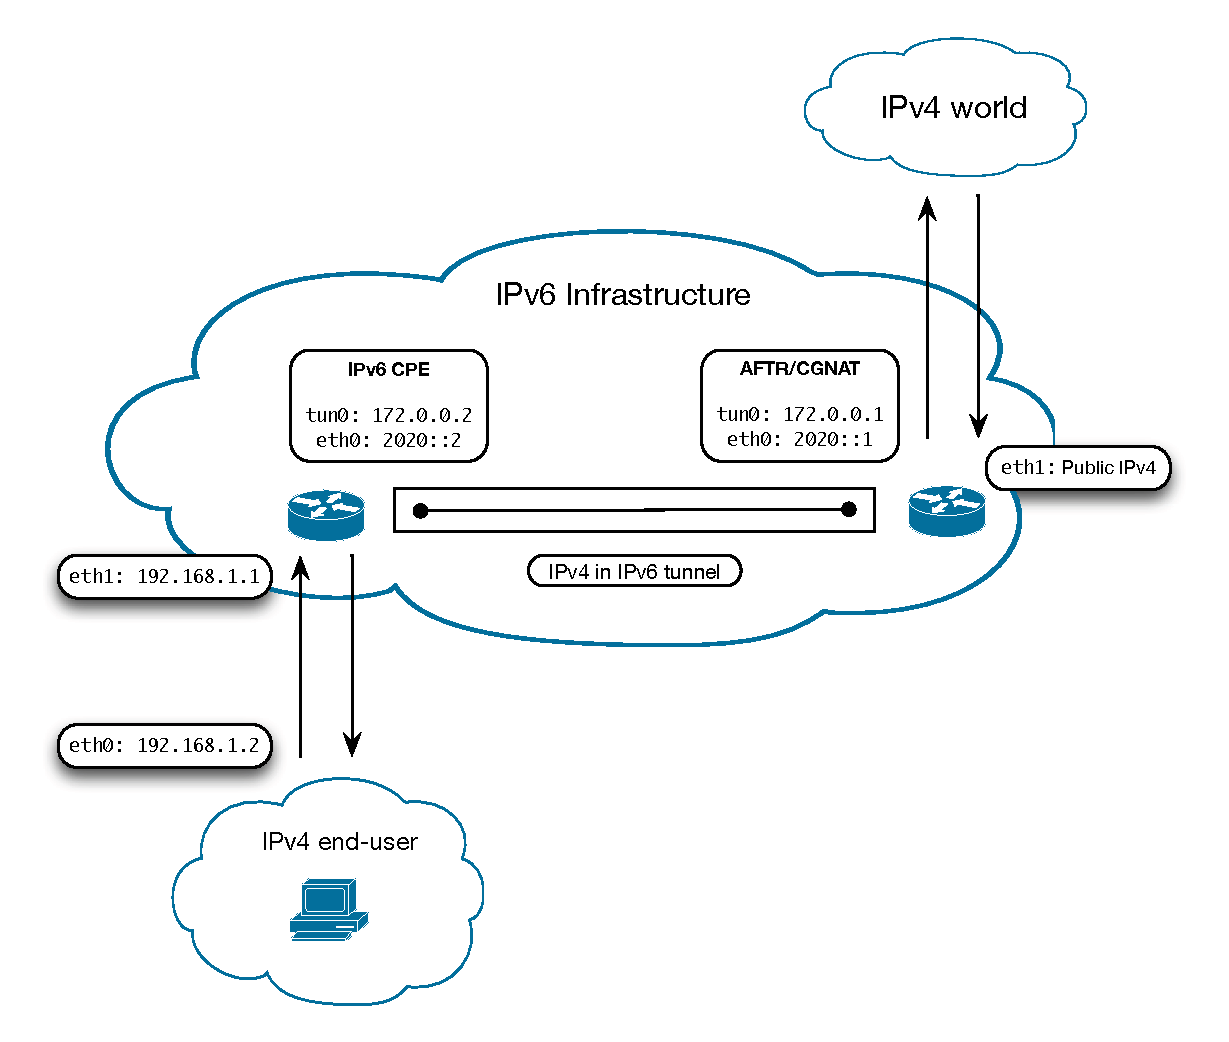
\includegraphics[scale=0.55]{dslite-setup}	
  \caption{Experimental Dual-Stack Lite setup}
  \label{fig:DSLiteSetup}
\end{figure}
We used three physical machines in our Dual-Stack Lite setup. One of the Debian machine works as our CPE, one as our CGNAT and the third one as our IPv4 only host running Mac OS X as shown in Figure \ref{fig:DSLiteSetup}. The CGNAT machine is a combination of an IPv4-in-IPv6 tunnel end-point and an IPv4-IPv4 NAT implemented on the same node \cite{DSLITE}. The machine has two interfaces, one (on \texttt{eth0}) with a Global Scope IPv6 address (\texttt{2020::1}) to underpin the virtual IPv4-in-IPv6 tunnel and the other one (on \texttt{eth1}) with a public IPv4 address to reach the IPv4 infrastructure. A virtual interface (\texttt{tun0}) was defined with an IPv4 address (\texttt{172.0.0.1}) on top of \texttt{eth0} to establish an \texttt{ipip6} tunnel to the CPE. At this point, all \texttt{172.0.0.0/64} traffic was routed to \texttt{tun0} and all \texttt{2020::/64} traffic was routed to \texttt{eth0}. We used \texttt{iptables} to forward all the traffic from \texttt{tun0} to \texttt{eth1} and to allow NATing with the public IPv4 address. We also enabled IPv4 forwarding on all interfaces for the \texttt{iptables} forwarding to work. 

The CPE machine is an IP router in the customer premise functioning as a home gateway that is connected to the service provider network. The B4 element \cite{DSLITE} implemented on a Dual-Stack capable node within the CPE creates a tunnel to route all IPv4 requests to the CGNAT machine. The machine has two interfaces, one \texttt{(eth0)} with a Global Scope IPv6 address (\texttt{2020::2}) to underpin the virtual IPv4-in-IPv6 tunnel similar to the CGNAT machine, and the other one \texttt{(eth1)} with a private \cite{RFC1918} address \texttt{(192.168.1.1)} which serves as the DHCP server for IPv4 clients directly connected to it. We added a default route for all IPv6 packets to pass through \texttt{eth0} with \texttt{2020::1} (CGNAT) as their next hop. At this point we could test IPv6 connectivity from both endpoints. A virtual interface (\texttt{tun0}) was defined with an IPv4 address (\texttt{172.0.0.2}) on top of \texttt{eth0} to establish an \texttt{ipip6} tunnel to the CPE. 
We added a default route for all IPv4 packets to pass through this virtual tunnel. At this point we could test IPv4 connectivity of tunnel endpoints. We also added a specific route for our private subnet \texttt{192.168.0.0/16} to route all local traffic through to \texttt{eth1}. We again used \texttt{iptables} to forward all the traffic, but this time from \texttt{eth1} to \texttt{tun0} and to allow NATing with the tunnel's IPv4 address \texttt{(172.0.0.2)}. We also enabled IPv4 forwarding on all interfaces for the \texttt{iptables} forwarding to work. 

The IPv4 only host has one interface \texttt{eth0} with a private address. A default IPv4 route was added on this machine to send all its IPv4 requests to the CPE. At this point we could test its IPv4 connectivity with the IPv4 world. 

\begin{table}[ht!]
  \centering
  \caption{Applications and services tested with DS-Lite and NAT64}
  \begin{tabular}{|ll|}
    \hline
    \multicolumn{2}{|l|}{Safari 5, Google Chrome 10, Firefox 4, Opera 11} \\
    ~~~- & WebMail: Gmail using TLSv1 \\
    ~~~- & Media: YouTube using Flash and HTML5 \\
    ~~~- & Google Maps, HTTP Downloading \\
    ~~~- & Web Chat: Gmail, Yahoo, Freenode IRC \\
    \hline
    \multicolumn{2}{|l|}{Miscellaneous} \\
    ~~~- & SSH, FTP, IRC, Git, Mercurial, OpenVPN \\
    ~~~- & Transmission: Bit Torrent \\
    \hline
  \end{tabular}
  \hfill
  \begin{tabular}{|ll|}
    \hline
    \multicolumn{2}{|l|}{Apple Mail 4} \\
    ~~~- & IMAP: Gmail and Microsoft Exchange \\
    ~~~- & POP3: Gmail \\
    ~~~- & SMTP: Gmail and Microsoft Exchange \\
    \hline
    \multicolumn{2}{|l|}{Instant Messaging and VoIP} \\
    ~~~- & iChat \\
    ~~~- & Skype \\
    ~~~- & SIP \\
    \hline
  \end{tabular}
  \label{tab:tests}
\end{table}

Once the setup of DS-Lite was performed, we carried out a number of application evaluations. As such, we ran the set of applications and protocols listed in Table~\ref{tab:tests}. Contrary to our expectations, we were not able to identify any failures. All of these installed applications worked out-of-the-box. Since there were no failures, we naturally could not define any failure signatures as well. Later, we evaluated NAT64 on the same set of applications, and observed different results as described in the next section.

\section{Testing NAT64}
\label{sec:app-nat64}

The NAT64/DNS64 experimental setup is shown in Figure \ref{fig:NAT64Setup}. A Debian machine functions as our IPv6 only host. It has one interface with one global scope IPv6 address to directly reach the IPv6 world and another global scope IPv6 address to reach the IPv4 world using NAT64. Another Debian machine, located within the same subnet as the IPv6 only host, functions as our DNS64 server to which our IPv6 only host sends all DNS queries. To achieve this, our IPv6 only host defines the DNS64 server as the only name-server. In order to process all IPv6 DNS requests, \texttt{totd} \cite{TOTD} was installed on the DNS64 server, which is a stateless user-space implementation of DNS64 which forwards the requests to a real IPv4 name-server and then constructs fake IPv6 address based on a pre-defined IPv6 NAT64 prefix (\texttt{64:FF9B::}) and the IPv4 address received from the IPv4 name-server answering the DNS request.

The NAT64 machine runs Debian and has two network interfaces. One of the interfaces (\texttt{eth0}) has a public IPv4 address and is connected to the IPv4 world. The other interface ({\texttt{eth1}}) has a Global Scope IPv6 address to connect back to our IPv6 only host. In order to route all IPv6 requests with a NAT64 prefix (\texttt{64:FF9B::}) to the NAT64 machine, a default route was setup on the IPv6 only machine. In order to get the IPv6-IPv4 translation working, we installed \texttt{Ecdysis} \cite{ECDYSIS}, which is an open-source implementation of NAT64 to translate all IPv6 packets received at \texttt{eth1} (from the IPv6 only machine) to IPv4 packets and to send them via the \texttt{eth0} interface to the IPv4 infrastructure. At this point we could access IPv4 websites from our IPv6 only host. Since, our IPv6 only host is also directly connected to the IPv6 infrastructure, we were also able to reach IPv6 only websites.

\begin{figure}[t!]	
  \centering
  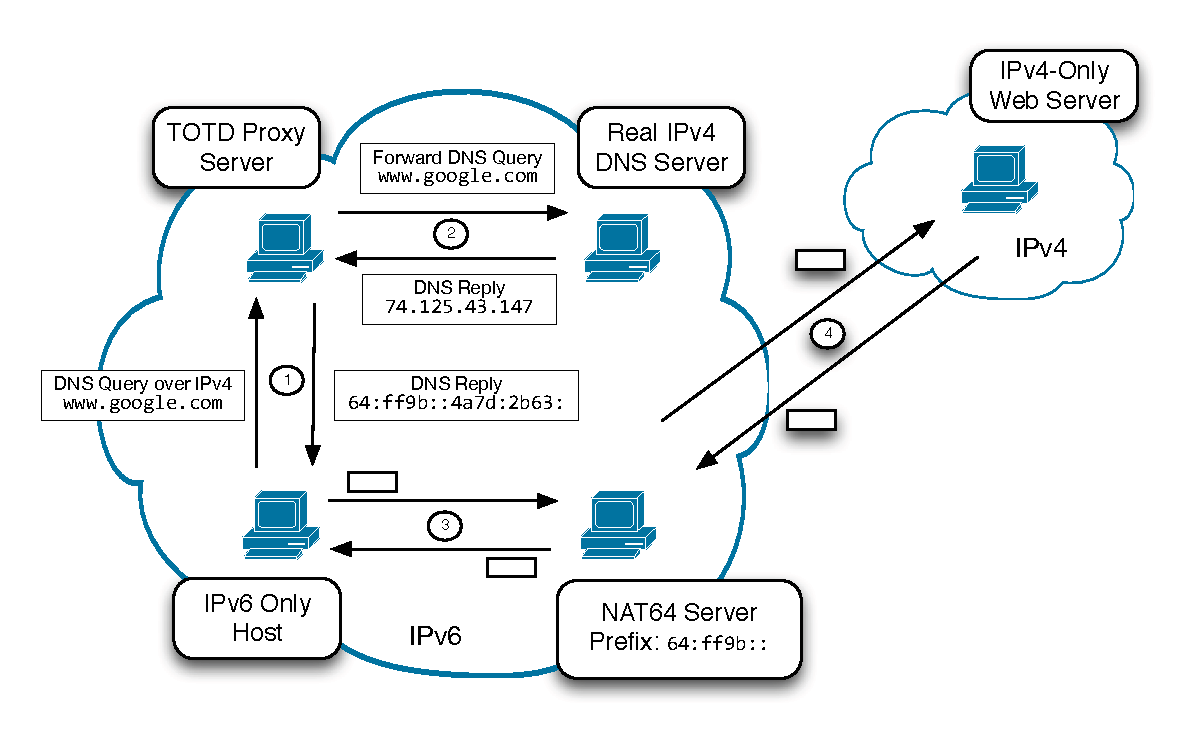
\includegraphics[scale=0.60]{nat64-setup}	
  \caption{Experimental NAT64/DNS64 setup}
  \label{fig:NAT64Setup}
\end{figure}

We tested the same set of applications and protocols as presented in
Table~\ref{tab:tests}. For the majority of applications the experiences have been similar to those of DS-Lite. However, four of the applications failed to interoperate with NAT64: Skype, OpenVPN, Transmission (bit-torrent) and SIP clients. In the next section we discuss the reasons for failure of these applications.

\section{Failure Analysis}
\label{sec:failure-analysis}

These failures correspond to similar experiences with NAT64, documented in other independent studies \cite{ARKKO, UENO,   citeulike:9731000}. Skype, for instance has its own unique behavior during the startup and sign-in procedure. At the start of the sign in procedure, Skype tries to discover clients in the local network. It tries to send a multicast message using the multicast DNS (mDNS) protocol. To perform that, it uses a specific IPv4 multicast address and mDNS port \texttt{(224.0.0.251:5353)} combination. On an IPv6-only host, this phase obviously fails. With the start of the second phase, Skype tries to establish contact to the Skype login server. The login server resides on an IPv4 address, but that address is mapped into an IPv6 address by the DNS64 server. There are three subsequent attempts with increasing duration and decreasing number of packets to establish contact with the login server. However, each attempt fails owing to the lack of IPv6 support in the Skype client.

There are applications with partial IPv6 support, but they fail to operate without a dual-stacked environment. Transmission, a bit-torrent client, for instance, could successfully connect to the tracker of the torrent file and retrieve the list of peers and seeders. However, it failed to connect to any of the peers when the client ran on an IPv6-only host. OpenVPN is another such example where the client failed to transport VPN packets over IPv6. Obviously, applications failing to generate sufficient amounts of traffic due to incomplete IPv6 support are difficult to identify using flow records.

Linphone, a SIP client with well-recognized IPv6 support, showed potential to be a candidate for defining failure signatures. To be able to identify behavior which would be unique to SIP clients, we decided to capture and analyze the transmissions at the packet-level using WireShark. The NAT64 box was chosen as the monitoring point since it was the best place to get a perspective from both ends of the network. We observed that the client initially tried to register with ekiga.net using its IPv6 address and port number 5060, but received a 606 error, which means that agent was recognized successfully but some aspects of the session description (addressing style) were not accepted \cite{rfc3261}. The 606 error response, however, also contained the public IPv4 address of the NAT64 box, which was used as a source in the subsequent \texttt{REGISTER} requests by the agent. This second attempt eventually succeeded and resulted in a \texttt{OK} (200) response code in the SIP reply. During call initiation, different behaviors were observed for both incoming and outgoing calls from the IPv6-only host. An outgoing call showed up expected behavior, with an \texttt{INVITE}, triggering a \texttt{TRYING} (100), \texttt{RINGING} (180) and eventually an \texttt{OK} (200) response from the other end. An incoming call on the other hand led to two additional responses from the IPv6-only host just after receiving an \texttt{INVITE}, namely \texttt{Dialog Establishment} (101) and an \texttt{OPTIONS} packet \cite{rfc3261}. In both cases, however, while the SIP signaling works out correctly, the call itself does fail. This is due to IPv4 address literals carried in SDP records identifying the endpoints for the voice streams.

After having learned the reason why SIP clients fail, we looked at the identification of the failure at the flow-level. We defined a sample config file with a flow-template containing 5 keys (srcIP, dstIP, srcPort, dstPort, protocol) and 2 aggregation elements (packetCount, totalBytes). Setting an appropriate export time to segregate the flows was a challenge, whereby a large number smeared all packets into a single flow, while a lower value diverged the related packets in separate flows making them less useful. It would have been possible to get an appropriate value looking at the WireShark traces, but then that value would correspond to a specific scenario, and thus could not be used as a general case study. Furthermore, it was difficult to clearly distinguish session initiation or teardown SIP exchanges from registration exchanges. Since SIP registrations establish soft state, they need to be renewed periodically. While certain implementation use known defaults for the timeouts, there is nothing suggested or even mandated in the SIP specification and thus registration traffic is implementation specific. Furthermore, users starting a VoIP client only when they place calls will have the registration traffic very likely merged with the call initiation traffic into a single flow record.

Another challenge is the identification of the absence of RTP flows between call initiation and call teardown. Note that there are no fixed port numbers for RTP \cite{rfc3551}. The reserved port numbers may be used by applications, but applications are essentially free to use any ephemeral port. Hence, any UDP flow matching the start and end times could be a possible RTP stream. Looking at the traffic characteristics of the UDP flows also is of minor value. While some traditional codecs lead to more or less constant bitrate flows, smarter more recent codecs may not send traffic at all if there is no audio signal to carry. Hence, our attempts to formulate failure signatures as NFQL queries did lead to queries that are very client specific and which can easily produce a high number of false positives. It is likely that we could have produced sharper queries if the flow records would contain more details about the protocol exchanges taking place. For example, if the flow records would indicate which SIP methods were invoked during the time interval covered by a flow record, we would have been able to match UDP flows more easily. Furthermore, if the UDP flows have been tagged as RTP flows, we could have easily ignored other UDP flows. As such, Flexible NetFlow \cite{flexiblenetflow:2008} with its packet section export capability to allow deep packet inspection of flow-records can serve as a good candidate to identify this behavior and is a potential item for future work.

\section{Related Work}
\label{sec:related-ipv6}

A number of technologies, besides NAT64 and DS-Lite have also been proposed that attempt to provide their perspective on how to go about this transition. The author of \cite{GEOFFAPNIC} provides a detailed discussion on these technologies. For instance, TAYGA \cite{TAYGA} is a user space stateless NAT64 implementation for Linux that uses the \texttt{tun} driver to exchange IPv4 and IPv6 packets with the kernel. It is intended to provide production-quality NAT64 service for networks where dedicated NAT64 hardware would be an overkill. Routing TAYGA's IPv4 path through a stateful NAT44 can also make it stateful. 

Address Plus Port [A+P] \cite{AP} is another transition technology that uses a NAT in (or close to) the customer premise for access to the IPv4 Internet. The Service Provider conveys both an IPv4 address (as done today) and a range of TCP/UDP ports to the NAT. Outgoing IPv4 traffic is NAT'ed to that range of TCP/UDP ports, and the Service Provider routes packets to the appropriate customer using both the destination IPv4 address (as done today) and destination TCP/UDP port. This way, a global IPv4 address can be shared between multiple customers and there is only a single NAT involved.

NAT444 \cite{NAT444} is very similar to Dual-Stack Lite, however, it has an advantage of not imposing any special requirement on the CPE. It uses two IPv4 NATs and three layers of addressing instead of an IPv4-in-IPv6 tunnel. One layer uses a private IPv4 block behind the CPE, another uses a separate private IPv4 block between the CPE and CGNAT, and the third layer uses a public IPv4 address routing outside from the CGNAT to the IPv4 world.

Teredo \cite{TEREDO} is a technology to provide IPv6 connectivity to IPv4 endpoints whose service providers have not deployed IPv6 yet. Teredo is a platform-independent tunneling protocol designed to provide IPv6 connectivity by encapsulating IPv6 packets within IPv4 User Datagram Protocol (UDP) datagrams that can pass through NAT devices. Other Teredo nodes elsewhere, called Teredo relays, have access to the IPv6 network then receive the packets and route them on.

\section{Conclusion}
\label{sec:conclusion}

We investigated failures caused by IPv6 transition technologies and whether they can be detected in network flow records by defining failure signatures. Using such signatures, an interested ISP could automatically identify failures and customers that might experience problems while rolling out IPv6 transitioning technologies. We tested a variety of applications and protocols under DS-Lite and NAT64. All of the tested applications performed well with DS-Lite while some problems occurred with NAT64. We identified four applications that failed to function with our NAT64 setup and we carried out an analysis to identify as to what causes the applications to fail. However, with an
apparent lack of IPv6 support in three of them, it made little sense to define failure signatures since there is only a very small amount of traffic that can be observed (if any). Linphone, the fourth application with full IPv6 support, was analyzed at both the packet and flow level. It turned out that VoIP failures with NAT64 are difficult to identify in flow records due to the aggregation of traffic inherent in network flow records and the difficulty to identity the SIP methods being invoked and the lack of precision with which UDP flows can be classified as RTP flows. For our approach, it seems necessary that flow exporters provide more information about the application protocols carried in network flows.

\bibliographystyle{splncs}
\begin{thebibliography}{10}

\bibitem{ipv6monitor}
{IPv6 Adoption Monitor}.
\newblock \url{http://ipv6monitor.comcast.net/}, [Online; accessed
  10-February-2012].

\bibitem{APNIC}
{APNIC IPv4 Address Pool Reaches Final /8}.
\newblock \url{http://www.apnic.net/publications/news/2011/final-8}, [Online;
  accessed 10-February-2012].

\bibitem{iana}
{Available Pool of Unallocated IPv4 Internet Addresses Now Completely Emptied}.
\newblock \url{http://www.icann.org/en/news/releases/release-03feb11-en.pdf},
  [Online; accessed 10-February-2012].

\bibitem{ARKKO}
J.~Arkko and A.~Keranen.
\newblock {Experiences from an IPv6-Only Network}.
\newblock Internet-Draft (draft-arkko-ipv6-only-experience-05), February 2012.

\bibitem{UENO}
H.~Hazeyama and Y.~Ueno.
\newblock {Experiences from an IPv6-Only Network in the WIDE Camp Autumn 2011}.
\newblock Internet-Draft (draft-hazeyama-widecamp-ipv6-only-experience-00),
  October 2011.

\bibitem{citeulike:9731000}
N.~Skoberne and M.~Ciglaric.
\newblock {Practical Evaluation of Stateful {NAT64}/{DNS64} Translation}.
\newblock {\em Advances in Electrical and Computer Engineering}, 11(3):49--54,
  2011.

\bibitem{MARINOV}
Vladislav Marinov and J{\"{u}}rgen Sch{\"{o}}nw{\"{a}}lder.
\newblock {Design of a Stream-Based IP Flow Record Query Language}.
\newblock In {\em Proceedings of the 20th IFIP/IEEE International Workshop on
  Distributed Systems: Operations and Management}, DSOM '09, pages 15--28,
  Berlin, Heidelberg, 2009. Springer-Verlag.

\bibitem{AIMS2010}
Kaloyan Kanev, Nikolay Melnikov, and J{\"{u}}rgen Sch{\"{o}}nw{\"{a}}lder.
\newblock {Implementation of a Stream-based IP Flow Record Query Language}.
\newblock In {\em Proceedings of the 4th International Conference on Autonomous
  Infrastructure, Management and Security}, AIMS'10, pages 147--158, Berlin,
  Heidelberg, 2010. Springer-Verlag.

\bibitem{DSLITE}
A.~Durand, R.~Droms, J.~Woodyatt, and Y.~Lee.
\newblock {Dual-Stack Lite Broadband Deployments Following IPv4 Exhaustion}.
\newblock RFC 6333, August 2011.

\bibitem{RFC1918}
Y.~Rekhter, B.~Moskowitz, D.~Karrenberg, G.~J. de~Groot, and E.~Lear.
\newblock {Address Allocation for Private Internets}.
\newblock RFC 1918 (Best Current Practice), February 1996.

\bibitem{NAT64}
M.~Bagnulo, P.~Matthews, and I.~van Beijnum.
\newblock {Stateful NAT64: Network Address and Protocol Translation from IPv6
  Clients to IPv4 Servers}.
\newblock RFC 6146, April 2011.

\bibitem{rfc6145}
X.~Li, C.~Bao, and F.~Baker.
\newblock {IP/ICMP Translation Algorithm}.
\newblock RFC 6145, April 2011.

\bibitem{DNS64}
M.~Bagnulo, A.~Sullivan, P.~Matthews, and I.~van Beijnum.
\newblock {DNS64: DNS Extensions for Network Address Translation from IPv6
  Clients to IPv4 Servers}.
\newblock RFC 6147, April 2011.

\bibitem{rfc3954}
B.~Claise.
\newblock {Cisco Systems NetFlow Services Export Version 9}.
\newblock RFC 3954, October 2004.

\bibitem{jschauer:thesis:2011}
Johannes Schauer.
\newblock {Flowy 2.0: Fast Execution of Stream based IP Flow Queries}.
\newblock Bachelor's thesis, Jacobs University Bremen, Campus Ring 1, 28759
  Bremen, Germany, May 2011.

\bibitem{JFALLEN}
James~F. Allen.
\newblock {Maintaining Knowledge about Temporal Intervals}.
\newblock {\em Communications of the ACM}, 26:832--843, November 1983.

\bibitem{TOTD}
{{The totd ('Trick Or Treat Daemon') DNS proxy}}.
\newblock \url{http://www.dillema.net/software/totd.html}, [Online; accessed
  10-Februrary-2012].

\bibitem{ECDYSIS}
Simon Perreault, Jean-Philippe Dionne, and Marc Blanchet.
\newblock {Ecdysis: Open-Source DNS64 and NAT64}.
\newblock In {\em AsiaBSDCon}, March 2010.

\bibitem{rfc3261}
J.~Rosenberg, H.~Schulzrinne, G.~Camarillo, A.~Johnston, J.~Peterson,
  R.~Sparks, M.~Handley, and E.~Schooler.
\newblock {SIP: Session Initiation Protocol}.
\newblock RFC 3261, June 2002.

\bibitem{rfc3551}
H.~Schulzrinne and S.~Casner.
\newblock {RTP Profile for Audio and Video Conferences with Minimal Control}.
\newblock RFC 3551 (Standard), July 2003.

\bibitem{flexiblenetflow:2008}
{Cisco IOS Flexible NetFlow Technology White Paper}.
\newblock White paper, Cisco Systems, September 2008.

\bibitem{GEOFFAPNIC}
Geoff Huston.
\newblock {Transitioning Protocols}.
\newblock {\em The Internet Protocol Journal}, 14(1):22--46, March 2011.

\bibitem{TAYGA}
{{TAYGA, Simple, No-fuss NAT64 for Linux}}.
\newblock \url{http://www.litech.org/tayga/}, [Online; accessed
  10-February-2012].

\bibitem{AP}
R.~Bush.
\newblock {The Address plus Port (A+P) Approach to the IPv4 Address Shortage}.
\newblock RFC 6346, August 2011.

\bibitem{NAT444}
I.~Yamagata, Y.~Shirasaki, A.~Nakagawa, J.~Yamaguchi, and H.~Ashida.
\newblock {NAT444}.
\newblock Internet-Draft (draft-shirasaki-nat444-05), January 2012.

\bibitem{TEREDO}
C.~Huitema.
\newblock {Teredo: Tunneling IPv6 over UDP through Network Address Translations
  (NATs)}.
\newblock RFC 4380, February 2006.

\end{thebibliography}
\end{document}
